\documentclass[]{article}
\usepackage[style=numeric,backend=biber,sorting=none]{biblatex}
\usepackage{graphicx}
\usepackage{float}
\addbibresource{references.bib}

% Title Page
\title{Financial Analysis Report}
\author{Mark Paveszka}


\begin{document}
\maketitle

\newpage

\begin{abstract}
\end{abstract}

\newpage

\tableofcontents

\newpage

\section{Introduction}
\paragraph{}
As a result of modern technology, the way things are done is very different compared how it was twenty years ago. Since then everything has been speeding up, including a key area of society, namely: education. In the past fifteen to twenty years several businesses emerged to make education better and easier for both students and teachers. These businesses usually try to create software artefacts to improve some aspect of the broader field. Such software artefacts are innovative learning tools and learning management systems (LMS). One of the most well-known companies in the education technology sector is Blackboard \cite{Blackboard_UK}. They provide several applications to improve the quality of teaching, but they are mostly known for Blackboard Learn \cite{Blackboard_Learn}, which is one of the most popular learning management systems currently available on the market. This fact is shown in Figure \ref{fig:LMS-2020} and Figure \ref{fig:LMS-2020-6-year}

\begin{figure}[H]
    \centering
    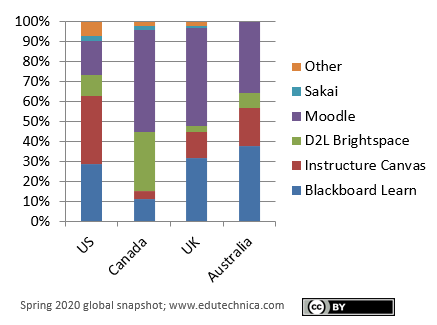
\includegraphics[width =\linewidth]{lms-vle-2020.png}
    \caption{LMS market share in 2020. \cite{VLE-2020-IMG}}
    \label{fig:LMS-2020}
\end{figure}

\begin{figure}
    \centering
    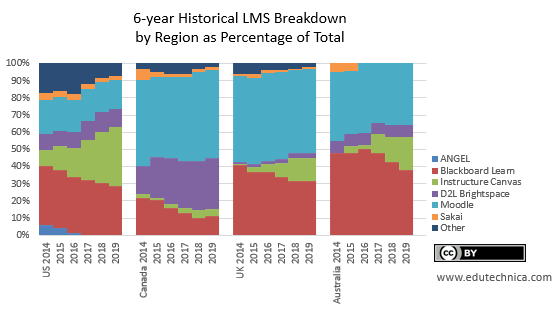
\includegraphics[width =\linewidth]{lms-vle-2020-y5.png}
    \caption{6-year historical LMS data by region. \cite{VLE-2020-IMG}}
    \label{fig:LMS-2020-6-year}
\end{figure}
\newpage
\section{Financial Analysis}

\newpage
\printbibliography{}

\end{document}          
